% Part: biographies % Chapter: bertrand-russell % Section: biography
\documentclass[../../../include/open-logic-section]{subfiles}

\begin{document}

\olfileid{bio}{ber}{bio} 
\olsection{Biography}
\begin{figure}[h!] 
\centering
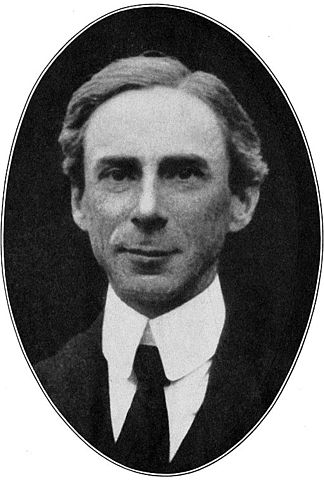
\includegraphics[scale=0.4]{bertrand-russell.jpg}
 \caption{Bertrand Russell. Photo Credit: Wikimedia.} 
\end{figure} 

Bertrand Russell is hailed
as one of the founders of modern analytic philosophy. Born May 18, 1872,
Russell was not only known for his work in philsoophy and logic, but wrote
many popular books in various subject areas. He was also an ardent
political activist throughout his life.

Russell was born in Trellech, Monmouthshire, Wales. His parents were
members of the British nobility. They were free-thinkers, and even made
friends with the radicals in Boston at the time \cite[9]{Russell1967}.
Unfortunately, Russell's parents died when he was young, and Russell was
sent to live with his grandparents. There, he was given a religious
upbringing (something his parents wanted to avoid at all costs)
\citep[11]{Russell1967}. His grandmother, although often liberal socially,
was very strict in all matters of morality \citep[15]{Russell1967}. During
adolesence he was mostly homeschooled by private tutors.

Russell's influence in analytic philosophy, and especially logic, is
tremendous. He studied mathematics and philosophy at Trinity College,
Cambridge, where he was influenced by mathematician Alfred North Whitehead.
In 1910, Russell and Whitehead published the first volume of
\emph{Principia Mathematica}, where they championed the view that
mathematics is reducible to logic. He then went on to publish major works,
such as his essay \emph{On Denoting} in 1905. He published 
hundreds of books, essays and political pamphlets during his time. He won
the Nobel Prize for literature in 1950.

Russell's life was filled with exciting and interesting events. He was
deeply entrenched in politics and social activism; during World War I he
was arrested and sent to prison for six months due to pacifist activities
and protest. While in prison, he was able to write and read, and claims to
have found the experience "quite agreeable" \citet[29]{Russell1968}. He
remained a pacifist throughout his life, and was again sent to jail for
attending a nuclear disarmorment rally in 1961. He also survived a plane
crash in 1948, where the only survivors were those sitting in the smoking
section. As such, Russell claimed that he owed his life to smoking. Russell
was also known to be a ladies man. He was married four times, but is
said to have had many extra-marital affairs.

Russel passed away on February 2, 1970 at the age of 97 in
Penrhyndeudraeth, Wales.

\begin{reading}

\begin{itemize}

\item Russell wrote an autobiography in three parts, spanning his life from
1872 - 1967. See \citet{Russel1967,Russel1968,Russell1969}.

\item The Bertrand Russell Research Centre at McMaster University is home
of the Bertrand Russell archives. See thier website at \citet{Duncan2015},
for information on the volumes of his
collected works (including searchable indexes), and archival projects.

\item Russell's paper \emph{On Denoting} is an important and interesting
read. See \citet{Russell1905}.

\item The Stanford Encyclopedia of Philosophy has sound clips of Russell
speaking on Desire and Political theory. See \citet{Irvine2015}.

\item Many video interviews with Russell are available online. To see him
talk about smoking and being involved in a plane crash, see
\citet{RussellND}.

\item Some of Russell's works, including his \emph{Introduction to
Mathematical Philosophy} are available as free audiobooks on
\citet{LibriVoxND}.

\end{itemize}

\end{reading}

\end{document}